
% this file is called up by thesis.tex
% content in this file will be fed into the main document

% ----------------------- introduction file header -----------------------
%\chapter{Search for the FCNC decay \pmb{$t\rightarrow c + Z$}}
\chapter{Search for the FCNC decay of top-quark in c-quark and Z boson}
\label{chapter:analysis}
This chapter presents a search for the Flavor-Changing-Neutral-Current decay of top-quark 
in c-quark and Z boson, denoted FCNC \textit{tZc}. The study uses a data sample of proton-proton collisions at 
$\sqrt{s}$= 13 TeV recorded in full Run2 (since 2015 to 2018) by the ATLAS experiment, and targets final states with three
leptons (either electrons or muons).
I took in charge most of the analysis, from the event selection up to the final results.
In particular, an important fraction of my work was dedicated to the event selection using the SMT technique and
the design and optimization of the multivariate analysis.
% ----------------------- paths to graphics ------------------------

% the code below specifies where the figures are stored
\graphicspath{Chapters/CH5/figures}

% ----------------------------------------------------------------------
% ----------------------- introduction content -------------------------
% ----------------------------------------------------------------------

\section{Physics motivation}
The heaviest particle in the Standard Model (SM), the top quark, decays almost exclusively to a $W$-boson and a bottom quark~\cite{pdg2}. In proton-proton ($pp$) collisions, top quarks are produced dominantly in pairs, via the strong interaction, but also singly, via the electroweak interaction. \\%involving a $Wtb$ vertex. %Therefore single-top quark production provides a powerful probe of the electroweak couplings of the top quark. 
Within the SM, flavour changing neutral currents (FCNC) processes are forbidden at tree level due to the Glashow-Iliopoulos-Maiani mechanism \cite{gim} and the approximate diagonality of the Cabibbo-Kobayashi-Maskawa matrix~\cite{pdg2} causes the suppression of such processes at higher orders. Nonetheless, there are several scenarios beyond the Standard Model (BSM) that can significantly enhance the FCNC processes in the top quark sector, opening a door for its detection at the Large Hadron Collider (LHC)~\cite{aguilar,barger,h2dm_limit,mssm_limit,RPV_limit, extra_limit}. \\
The analysis presented in the following searches for FCNC \textit{tZc} processes. A comparison between SM and BSM models predictions for the branching ratios of top quark decays to an up or a charm quark and a $Z$ boson is shown in Table \ref{tab:intro-fcnc-br-th}.\\

\begin{table}[h]
	\caption{The theoretical values for the branching ratios of FCNC top decays
		predicted by the SM, the quark singlet model (QS)~\cite{aguilar},
		the minimal supersymmetric standard model (MSSM)~\cite{mssm_limit}, SUSY with R parity violation
		(RPV SUSY)~\cite{RPV_limit} and warped extra dimensions (RS) (without prediction to up quark interactions) ~\cite{extra_limit} models.}
	\label{tab:intro-fcnc-br-th}
	\centering
	\begin{tabular}{l c c c c c}
		\toprule
		\textbf{Process} & SM & QS & MSSM & RPV SUSY & RS \\
		\midrule
		$t\to Zu$ & $10^{-17}$ & $\leq$ $10^{-4}$
		& $\leq$ $10^{-7}$
		& $\leq$ $10^{-6}$ & --\\
		$t\to Zc$ & $10^{-14}$ & $\leq$ $10^{-4}$
		& $\leq$ $10^{-7}$
		& $\leq$ $10^{-6}$ & $\leq$ $10^{-5}$\\
		\bottomrule
	\end{tabular}
\end{table}

\noindent The search for FCNC \textit{tZc} processes can be performed by analysing the top quark decays in $\mathrm{t\bar{t}}$ events as well as the production of single-top quarks (see Figure \ref{fig:signal}). In the former channel, one of the top quarks decays through FCNC and the other through the dominant mode ($t\to Wb$). The latter channel is characterised by a final state composed of a single top quark and a $Z$ boson. The main difference between the final state of decay and production modes is the presence of one additional jet. \\
The analysis presented in the following targets both production and decay mode. This search is done using $pp$ collision data collected by the ATLAS detector at a centre-of-mass energy of 13 TeV and corresponding to an integrated luminosity of 139 $\mathrm{fb^{-1}}$. The analysis targets both events with the production of a $Z$ boson and a single-top quark decaying to a $W$ boson and a b-quark and events with the production of top quark pairs, where one top quark decays to a $Z$ boson and a light quark (up or charm) and the other top quark decays to a $W$ boson and a b-quark. For both modes, the $Z$ boson decays into two charged leptons (electrons or muons including those coming from leptonic $\tau$-lepton decays) and the $W$ boson from the top quark decays leptonically too. \\

\begin{figure}[htb]
	\centering
	\subfigure[\textit{tZc} production via FCNC ($s$-channel)]{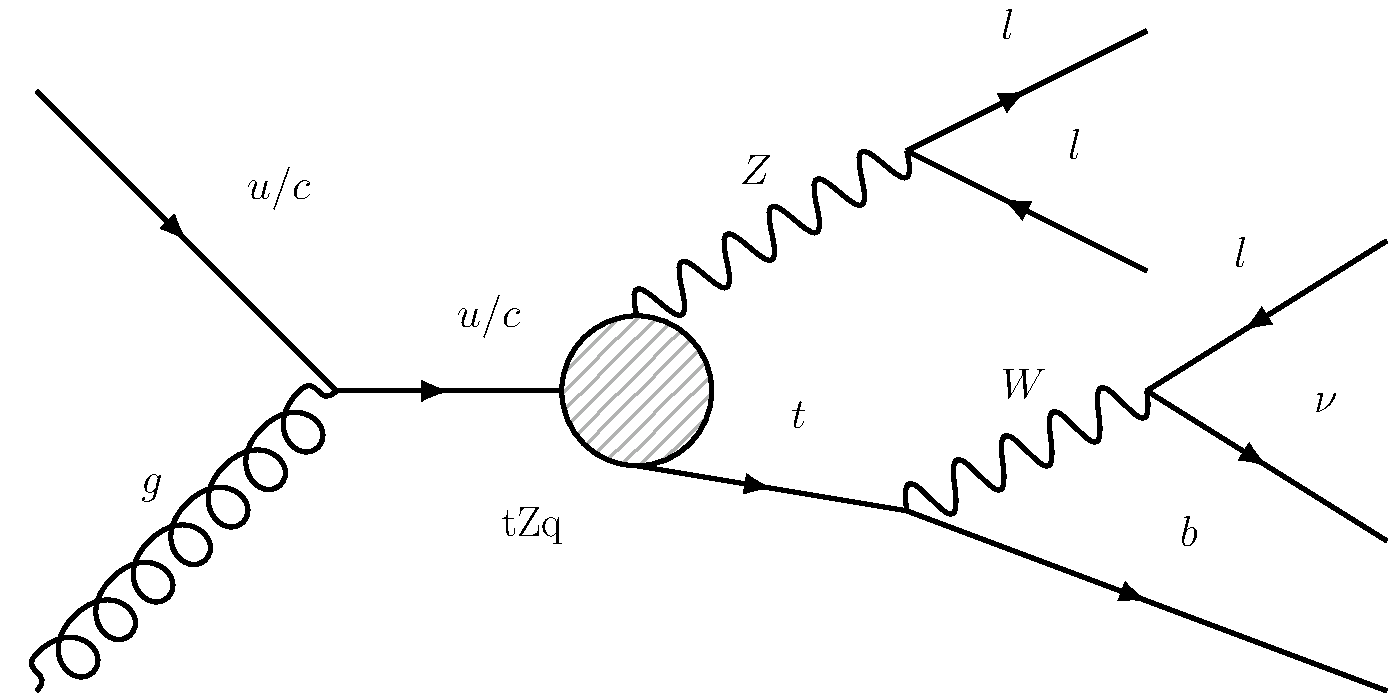
\includegraphics[width=0.50\textwidth]{Chapters/CH5/figures/Production_1.pdf}\label{subfig:signal1}}\qquad
	\subfigure[\textit{tZc} production via FCNC ($s$-channel)]{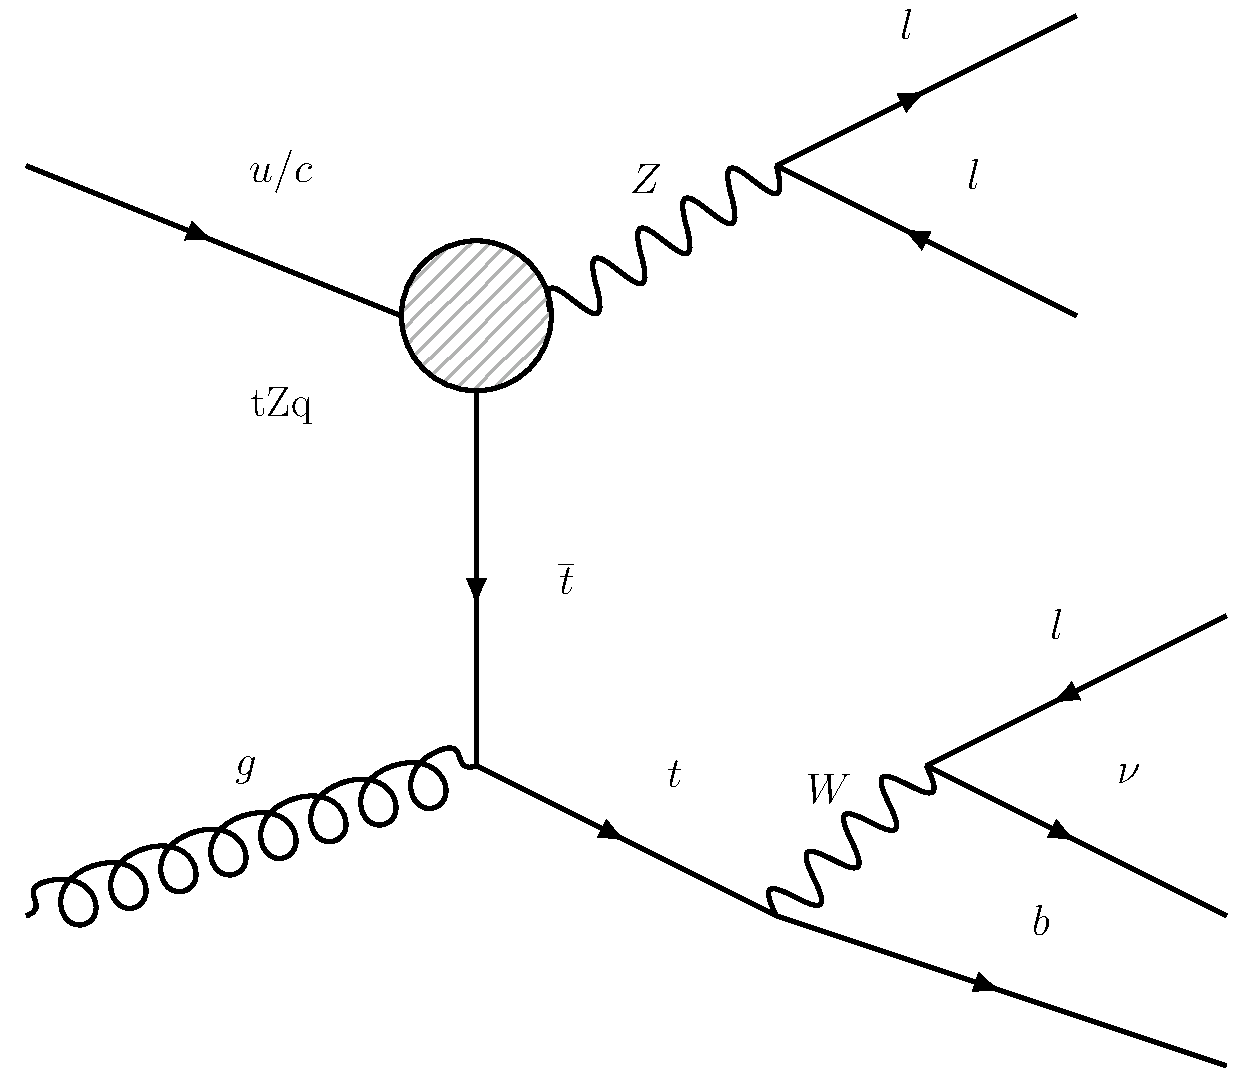
\includegraphics[width=0.40\textwidth]{Chapters/CH5/figures/Production_2.pdf} \label{subfig:signal2} }
	\subfigure[ $\mathrm{t\bar{t}}$ production with \textit{tZc} decay]{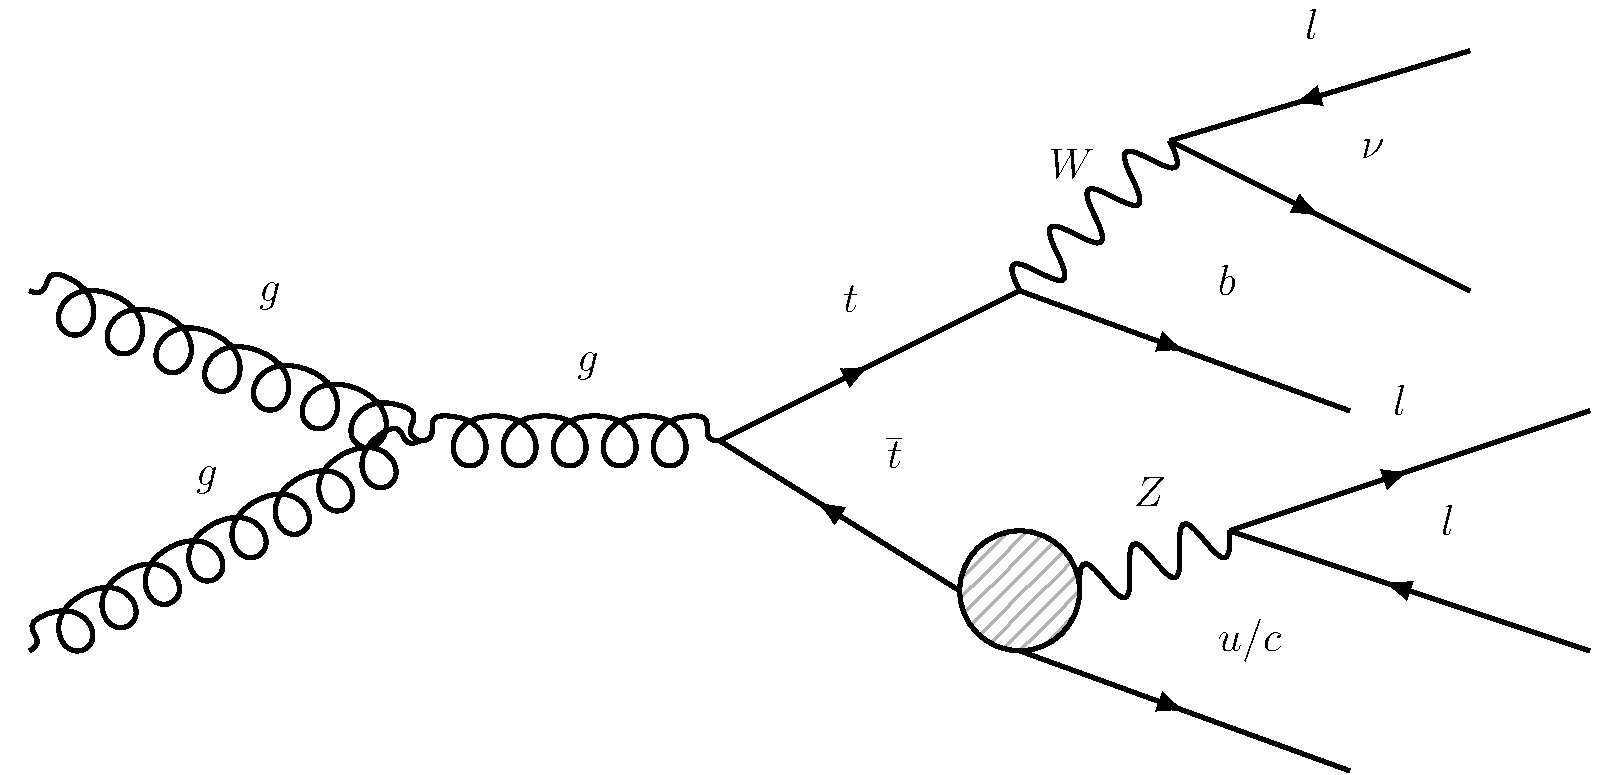
\includegraphics[width=0.54\textwidth]{Chapters/CH5/figures/TtbarProduction.pdf} \label{subfig:signal3}}
	\caption{Examples of lowest order Feynman diagrams for \textit{tZc} production via FCNC in \subref{subfig:signal1} the $s$-channel and \subref{subfig:signal2} the $t$-channel. Example of the lowest order Feynman diagrams for \subref{subfig:signal3} $\mathrm{t\bar{t}}$ production, with one top-quark decaying through the SM and the other via \textit{tZc}. The vertex labelled as \textit{tZq} corresponds to the coupling responsible for the FCNC interaction.}
	\label{fig:signal}
\end{figure} 

\noindent In a model independent way, the anomalous couplings can be described by the so called effective field theory (EFT).
This theory considers an extension of the SM Lagrangian $\mathcal{L}_{SM}$ by operators in higher-dimensions of the mass suppressed by the scale of new physics $\Lambda$ as shown in \cref{eq:lagrangian}.
Dimension-5 operators are not considered in this analysis due to the introduction of lepton-flavour violating processes. 
Therefore, the anomalous couplings can be approximated with dimension-6 operators $O_{i}^{(6)}$ whose strength  is given by the Wilson coefficients $C_{i}^{(6)}$.\\

\begin{equation}
\mathcal{L} = \mathcal{L}_{SM} + \frac{1}{\Lambda^2}\sum_{i} C_{i}^{(6)} O_{i}^{(6)}  
\label{eq:lagrangian}
\end{equation}

\noindent Experimental limits on the branching ratio of FCNC \textit{tZc} decays were previously established by experiments at the Large Electron-Positron Collider (LEP)~\cite{ALEPH,DELPHI,OPAL,L3}, the Hadron-Electron Ring Accelerator (HERA)~\cite{ZEUS}, the Tevatron\ \cite{CDF,DZero} and the Large Hadron Collider (LHC)~\cite{TOPQ-2017-06,Chatrchyan:2013nwa,CMS-TOP-12-039}. The ATLAS and the CMS collaborations obtained limits at the \SI{95}{\percent} confidence level (CL) for these processes using data collected at $\sqrt{s}$=\SI{13}{\TeV} and $\sqrt{s}$=\SI{8}{\TeV}, focusing on FCNC top-quark decays~\cite{TOPQ-2017-06,Chatrchyan:2013nwa}, or both production and decay modes combined~\cite{CMS-TOP-12-039}. 
A summary of the ATLAS and CMS results on the limits on FCNC couplings is shown in \cref{fig:intro:limits}. The actual observed limits on the FCNC \textit{tZc} couplings from ATLAS is $BR(t\to cZ) < \SI{2.4e-4}{}$~\cite{TOPQ-2017-06}.\\
Recent studies were done on the interference effects on the \textit{tZc} and $t\gamma q$ anomalous couplings, concluding that these effects are smaller than the variations of the systematics uncertainties considered~\cite{Interference}. Therefore, both decay and production modes are taken into account in this analysis to improve the results on the limits for \textit{tZc} anomalous couplings.

\begin{figure}[htb]
	\centering
	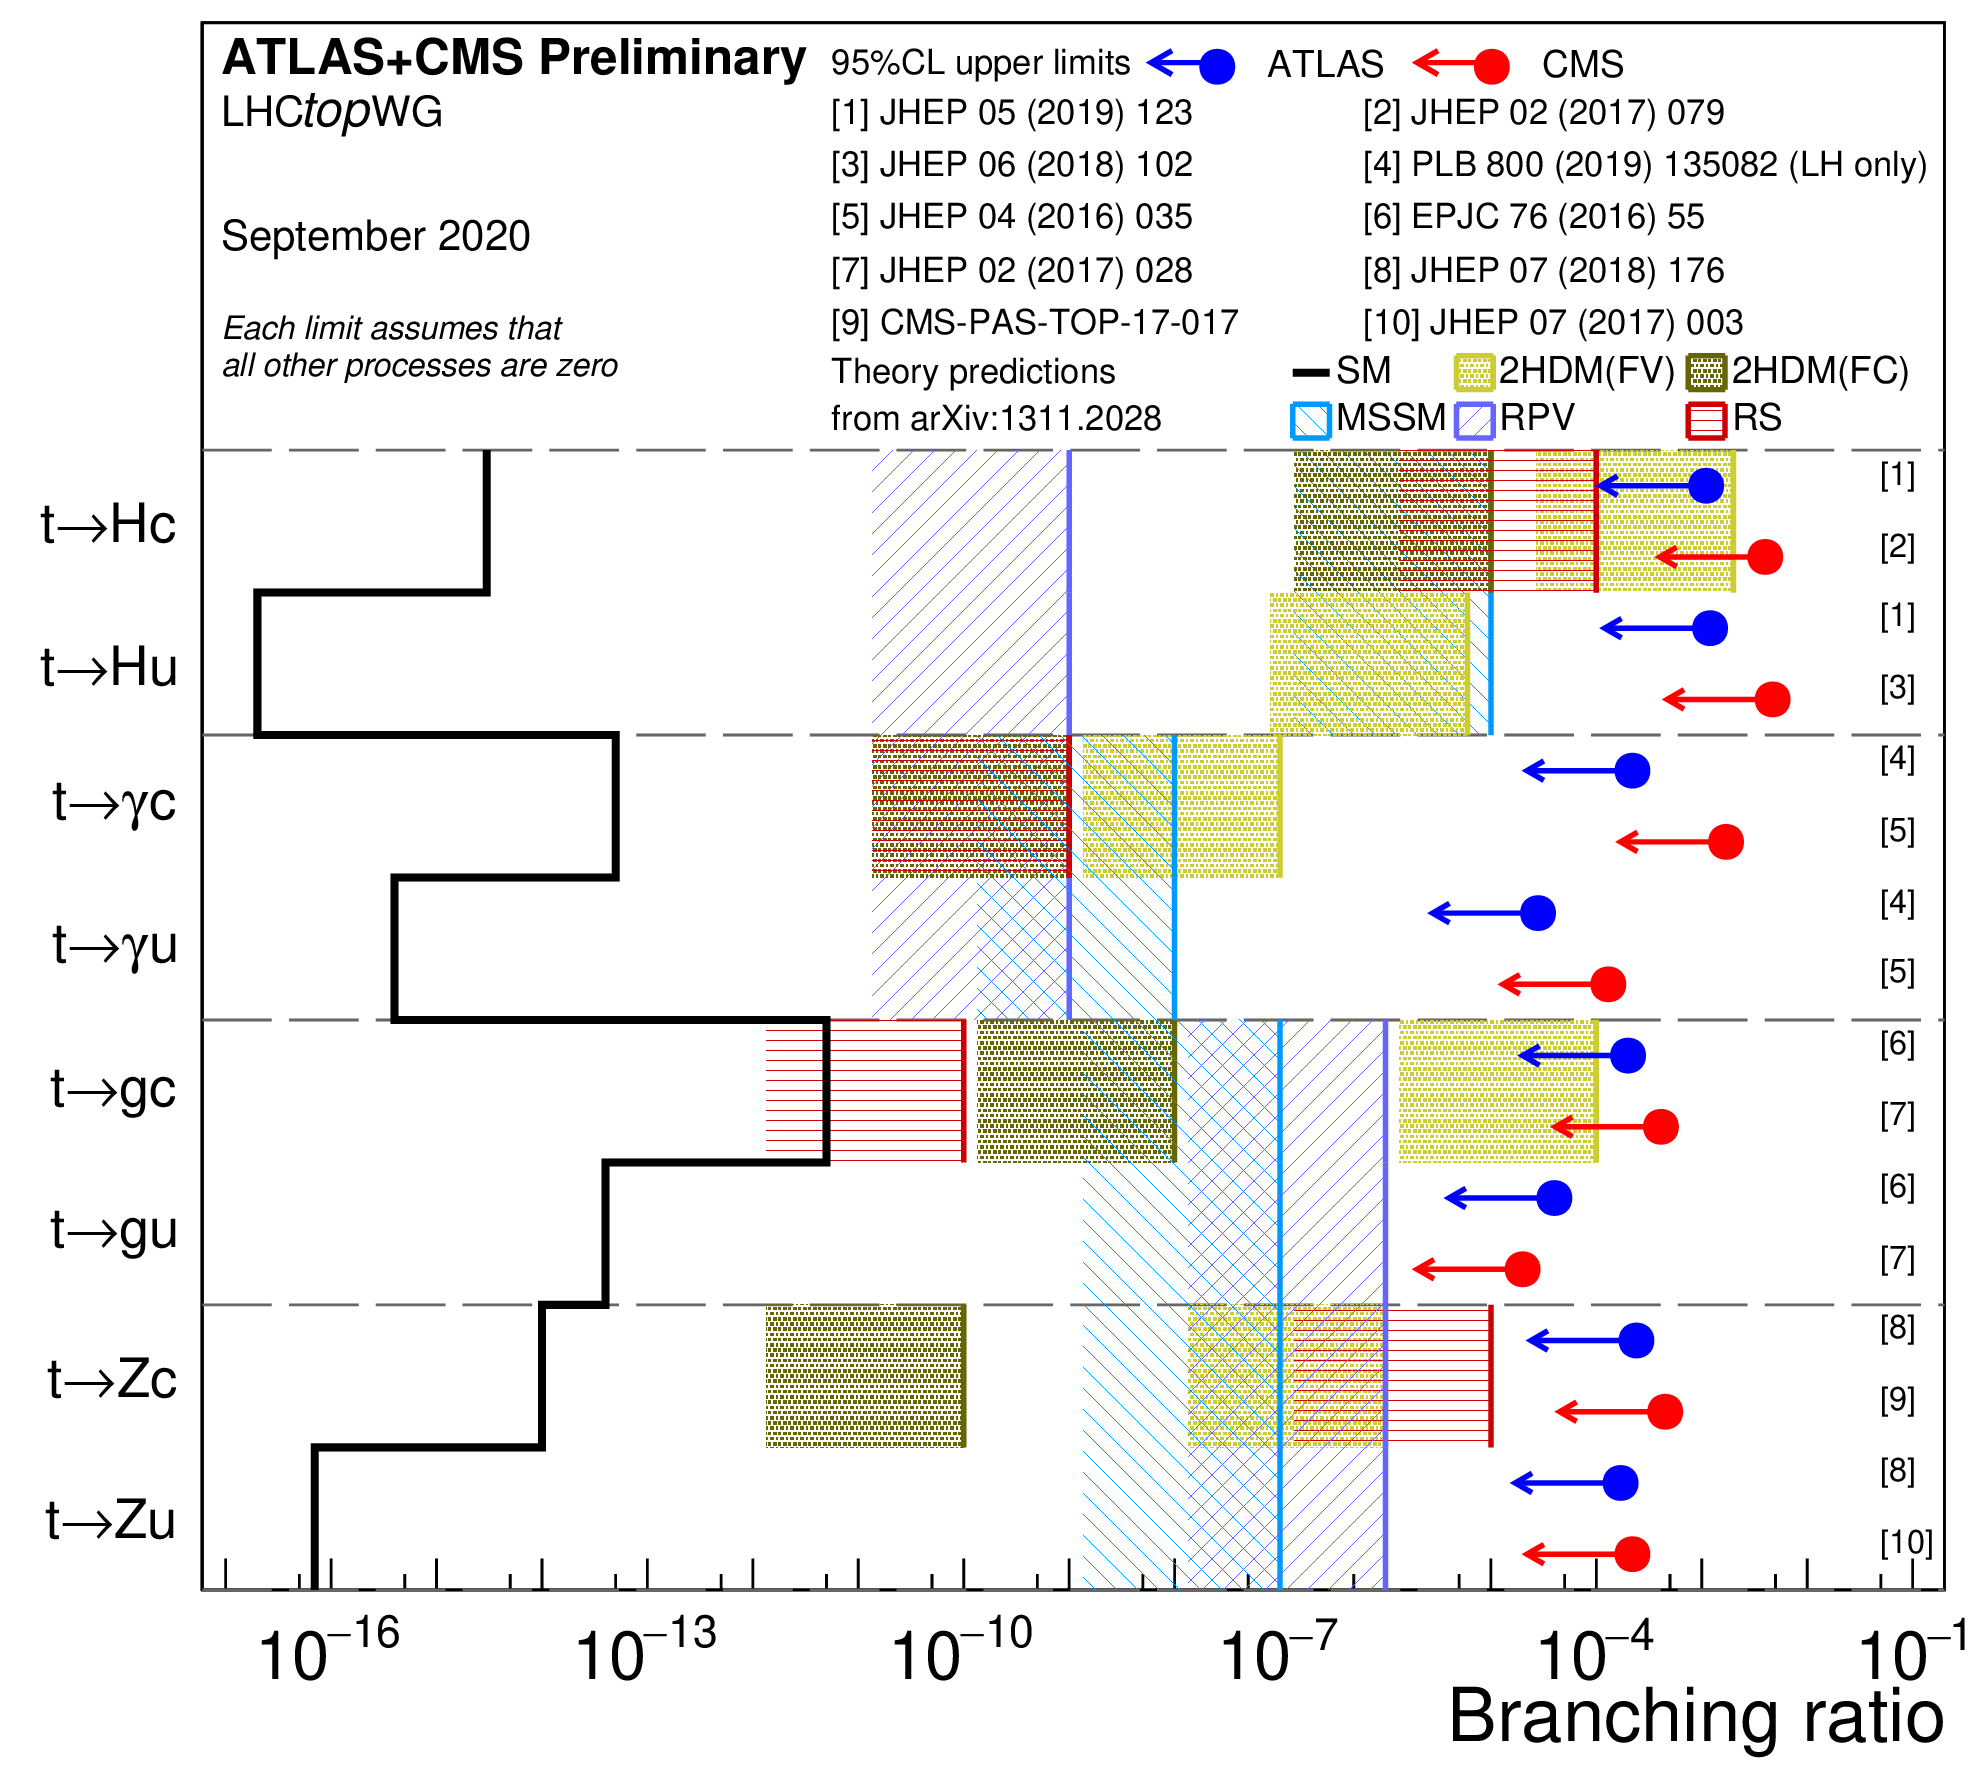
\includegraphics[scale=0.15]{Chapters/CH5/figures/fcnc_summarybsm}
	\caption{Summary of the current 95\% confidence level observed limits on the branching ratios of the top quark decays via flavour changing neutral currents to a quark and a neutral boson $t\rightarrow Xq$ ($X = g, Z, \gamma,$ or $H$; $q = u$ or $c$) by the ATLAS and CMS Collaborations compared to several new physics models. The ATLAS limits on $t \rightarrow q$ are valid for the case of a purely left-handed coupling. Status of figure: September 2019 (Top2019)}
	\label{fig:intro:limits}
\end{figure}

\clearpage
\section{Analysis strategy}

\clearpage
\section{Data and Monte Carlo samples}

\clearpage
\section{Event selections and reconstruction}
\begin{equation}
\chi^2=\frac{  (m^{reco}_{j_{SMT}l_{a}l_{b}} -m_{t_{FCNC}})^2 }{\sigma^2_{t_{FCNC}}}   +\frac{  (m^{reco}_{j_{bjet}l_{c}\nu} -m_{t_{SM}})^2 }{\sigma^2_{t_{SM}}}+\frac{  (m^{reco}_{l_{c}\nu} -m_{W})^2 }{\sigma^2_{W}}
\end{equation}
\clearpage
\subsection {Top quarks reconstruction}
\clearpage
\subsection {Signal Region definition}


\clearpage
\section{Background estimation}
\clearpage
\subsection {Control Regions definitions}
\clearpage
\subsection {Fake composition}



\clearpage
\section{Separation of signal from background events}
\clearpage
\subsection {GBDT discriminant definition}
\clearpage
\subsection {Input variables}
\clearpage
\subsection {GBDT training and evaluation}
\clearpage
\subsection {GBDT performance and over-training checks }


\clearpage
\section{Systematic uncertainties}
\clearpage
\subsection {Sources of systematic uncertainties}
\clearpage
\subsection {Acceptance and shape uncertainties}

\clearpage
\section {Additional Signal Regions and alternative c-tagger}
\clearpage
%\subsection {SR1 selections}
%\clearpage
%\subsection {SR2 selections}
%\clearpage
%\subsubsection {DL1r(c) selection}

